\documentclass{article}

\usepackage{hyperref}
\usepackage[T1]{fontenc}
\usepackage{graphicx}
\usepackage{float}
\usepackage[utf8]{inputenc}
\usepackage{amsmath}
\usepackage{amsfonts}


\title{%
Laboratorium 10\\
  \huge Równania różniczkowe - spectral bias}
\author{Mateusz Król}
\date{06/06/2024 r.}

\begin{document}
\maketitle

 
\section*{Zadanie 1.}
\textbf{Dane jest równanie różniczkowe zwyczajne
$$ \frac{du(x)}{dx} = cos(\omega x) \text{ dla } x \in \Omega \text{,}  $$
gdzie: \\
$x, \omega, u \in \mathbb{R}$,\\
x to położenie,\\
$\Omega$ to dziedzina, na której rozwiązujemy równanie, \\
$\Omega = \{x \text{  }| -2\pi \le x \le 2\pi\}$, \\
$u(\cdot)$ to funkcja, której postaci szukamy. \\\\
Warunek początkowy zdefiniowany jest następująco:
$$ u(0) = 0 \text{.}$$
Analityczna postać rozwiązania równania z warunkiem początkowym
jest następująca:
$$ u(x) = \frac{1}{\omega} \sin(\omega x) $$
Rozwiąż powyższe zagadnienie początkowe. Do rozwiązania użyj sieci neuronowych
PINN (ang. \textit{Physics-informed Neural Network} )
Można wykorzystać szablon w pytorch-u lub bibliotekę DeepXDE.\\\\
Warstwa wejściowa sieci posiada 1 neuron, reprezentujący zmienną $x$.\\
Warstwa wyjściowa także posiada 1 neuron, reprezentujący zmienną $\hat{u}(x)$.\\
Uczenie trwa przez $50 000$ kroków algorytmem \textit{Adam} ze stałą uczenia równą $0.001$.
Jako funkcję aktywacji przyjmij tangens hiperboliczny, $\tanh$.
}
\newpage

W poniższych rozwiązaniach wykorzystałem bibliotekę \textit{DeepXDE}.\\

Wykres rozwiązania zadanego równania różniczkowego dla danych modelu:\\
\begin{itemize}
  \item $\omega = 1$\\
  \item 2 warstwy ukryte, 16 neuronów w każdej warstwie\\
  \item liczba punktów treningowych: $200$\\
  \item liczba punktów testowych: $1000$
\end{itemize}

\begin{figure}[H]
  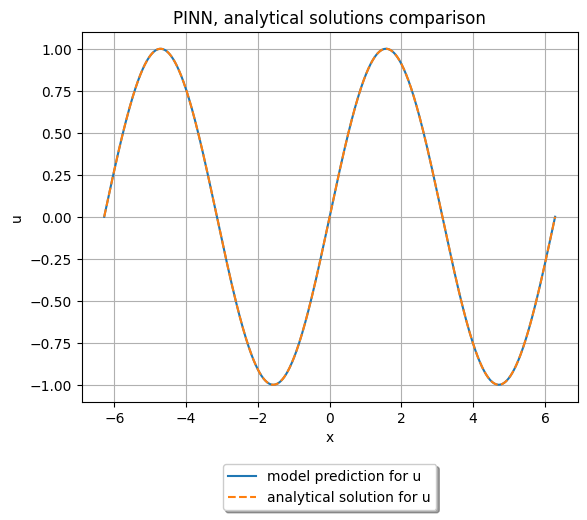
\includegraphics[width=\linewidth]{figures/first.png}
\end{figure}


Wykres rozwiązania zadanego równania różniczkowego dla danych modelu:\\
\begin{itemize}
  \item $\omega = 15$\\
  \item 2 warstwy ukryte, 16 neuronów w każdej warstwie\\
  \item liczba punktów treningowych: $3000$\\
  \item liczba punktów testowych: $5000$
\end{itemize}

\begin{figure}[H]
  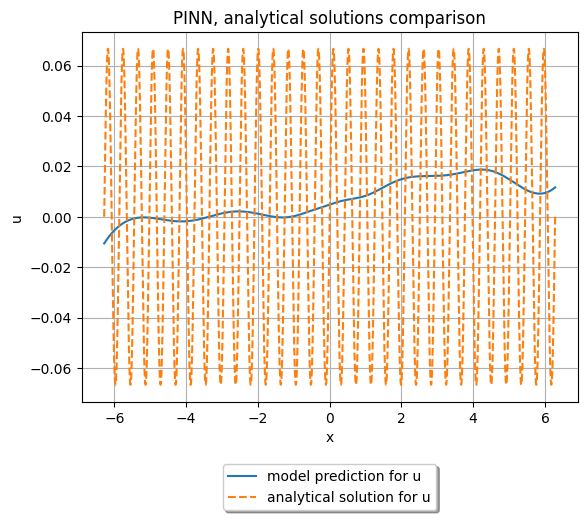
\includegraphics[width=\linewidth]{figures/second1.png}
\end{figure}

Wykres rozwiązania zadanego równania różniczkowego dla danych modelu:\\
\begin{itemize}
  \item $\omega = 15$\\
  \item 4 warstwy ukryte, 64 neuronów w każdej warstwie\\
  \item liczba punktów treningowych: $3000$\\
  \item liczba punktów testowych: $5000$
\end{itemize}

\begin{figure}[H]
  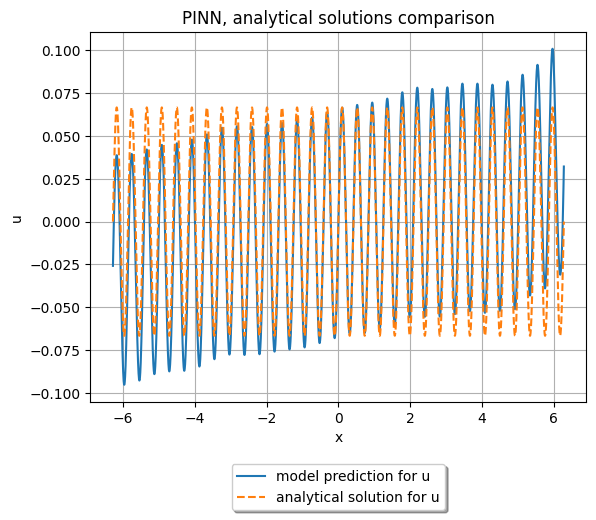
\includegraphics[width=\linewidth]{figures/second2.png}
\end{figure}

Wykres rozwiązania zadanego równania różniczkowego dla danych modelu:\\
\begin{itemize}
  \item $\omega = 15$\\
  \item 5 warstw ukrytych, 128 neuronów w każdej warstwie\\
  \item liczba punktów treningowych: $3000$\\
  \item liczba punktów testowych: $5000$
\end{itemize}

\begin{figure}[H]
  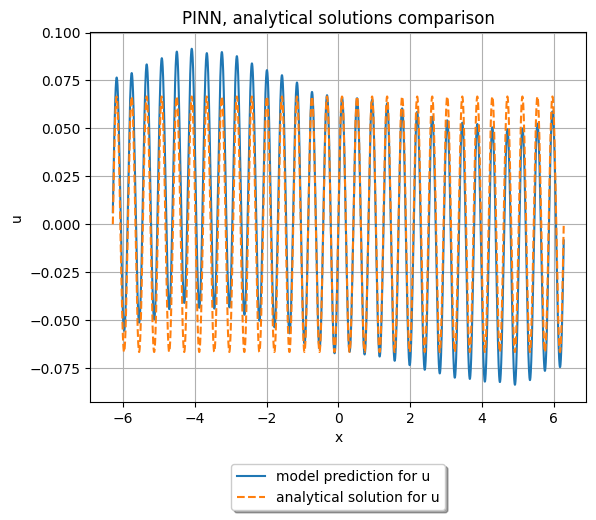
\includegraphics[width=\linewidth]{figures/second3.png}
\end{figure}



\end{document}